% ==============================================================================
% Universidade Federal do Rio Grande do Norte
% Centro de Tecnologia
% Programa de Pós-Graduação em Engenharia Elétrica e de Computação
% Qualificação
%
% Revisado em 12/07/2010 -- 10:00h
%
% Autor: Diogo Leite Rebouças <diogolr@gmail.com>
% ==============================================================================

% Classe .......................................................................
%\documentclass[a4paper,12pt,openright,twoside,notitlepage]{book}
\documentclass[a4paper,12pt,oneside,notitlepage]{book}

% Pacotes ......................................................................
% Pacotes Principais -----------------------------------------------------------
\usepackage[portuges,brazil]{babel}
\usepackage[utf8]{inputenc}

% Formatação de capítulos ------------------------------------------------------
%\usepackage[Sonny]{fncychap}
%\usepackage{fncychap}
\usepackage{capitulos}

% Figuras e Imagens ------------------------------------------------------------
\usepackage{graphicx}
% Figuras lado a lado
\usepackage{epsfig}
\usepackage{subfigure}

% Utilizar H para inserir as imagens REALMENTE onde eu desejo
\usepackage{float}

% Fontes -----------------------------------------------------------------------
\usepackage[T1]{fontenc}
\usepackage{pslatex}

% Simbolos ---------------------------------------------------------------------
\usepackage{textcomp}
\usepackage{bbding}

% Tabelas ----------------------------------------------------------------------
%\usepackage{multicol}
\usepackage{multirow}
% Colorir a tabela
\usepackage{colortbl}
% Pacote hhline corrige os bugs das linhas que não aparecem com o colortbm
\usepackage{hhline}
% Tabelas com colunas de largura auto ajustável
\usepackage{tabularx}
% Notas de rodapé em tabelas (Pode-se usar o ambiente longtable também -
% Pesquisar exemplo com longtable)
\usepackage{threeparttable}
% Tabelas grandes
\usepackage{supertabular}

% Glossário --------------------------------------------------------------------
\usepackage[portuguese,noprefix]{nomencl}
\usepackage{makeglo}

% Outros pacotes ---------------------------------------------------------------
\usepackage{noitemsep}
\usepackage{indentfirst}

% Comentários em bloco
\usepackage{verbatim}

% Hiperlinks
\usepackage{hyperref}

% Orientação de página
\usepackage{lscape}

% utilitários matemáticos
\usepackage{amsmath}
\usepackage{icomma}

% Evita o problema "too many unprocessed floats", colocando os campos
% 'flutuantes' em suas respectivas seções
\usepackage[section]{placeins}

% Highlight de códigos
\usepackage{minted}

% Referências ------------------------------------------------------------------
\usepackage[abbr]{harvard}	% As chamadas são sempre abreviadas
\harvardparenthesis{square}	% Colchetes nas chamadas
\harvardyearparenthesis{round}	% Parêntesis nos anos das referências
\renewcommand{\harvardand}{e}	% Substituir "&" por "e" nas referências


% Comandos .....................................................................
% Comandos gerais --------------------------------------------------------------
\newcommand{\titulo}{Título do trabalho grande o suficiente para ter uma ideia
                     do que irá acontecer na capa}
\newcommand{\autor}{Diogo Leite Rebouças}
\newcommand{\orientador}{Fábio Meneghetti Ugulino de Araújo}
\newcommand{\coorientador}{André Laurindo Maitelli}
\newcommand{\diaaprovacao}{26}
% Mês com inicial maiúscula (capa, folha de rosto)
\newcommand{\Mesaprovacao}{Julho}
% Mês com inicial minúscula (folha de assinaturas)
\newcommand{\mesaprovacao}{julho}
\newcommand{\anoaprovacao}{2010}
\let\Anoaprovacao\anoaprovacao
\newcommand{\dataaprovacao}{\diaaprovacao\ de \mesaprovacao\ de \anoaprovacao}

% Configuração da fonte
%\renewcommand{\familydefault}{\sfdefault}

% Margens ----------------------------------------------------------------------
\setlength{\oddsidemargin}{3.5cm}
\setlength{\evensidemargin}{2.5cm}
\setlength{\textwidth}{15cm}
\addtolength{\oddsidemargin}{-1in}
\addtolength{\evensidemargin}{-1in}

\setlength{\topmargin}{2.0cm}
\setlength{\headheight}{1.0cm}
\setlength{\headsep}{1.0cm}
\setlength{\textheight}{22.7cm}
\setlength{\footskip}{1.0cm}
\addtolength{\topmargin}{-1in}

% Glossário --------------------------------------------------------------------
\makeglossary

% Capítulos --------------------------------------------------------------------
% Não aparecer o número na primeira página dos capítulos
\newcommand{\mychapter}[1]{\chapter{#1}\thispagestyle{empty}}
\newcommand{\mychapterstar}[1]{\chapter*{#1}\thispagestyle{empty}}

% Comandos matemáticos ---------------------------------------------------------
% Implicação em fórmulas
\newcommand{\implica}{\quad\Rightarrow\quad} %Meio de linha
\newcommand{\implicafim}{\quad\Rightarrow}   %Fim de linha
\newcommand{\tende}{\rightarrow}

% Fração com parenteses
\newcommand{\pfrac}[2]{\parent{\frac{#1}{#2}}}

% Transformada de Laplace e transformada Z
\newcommand{\lapl}{\pounds}
\newcommand{\transfz}{\mathcal{Z}}

% Sequências
\newcommand{\sequencia}[4]{$#1_{#2}$, $#1_{#3}$, \ldots, $#1_{#4}$}

% Outros ----------------------------------------------------------------------
\newcommand{\chave}[1]{\left\{#1\right\}}
\newcommand{\colchete}[1]{\left[#1\right]}
\newcommand{\parent}[1]{\left(#1\right)}

% Hyperref ---------------------------------------------------------------------
\hypersetup{
    bookmarks=true,         % show bookmarks bar?
    unicode=false,          % non-Latin characters in Acrobat’s bookmarks
    pdftoolbar=true,        % show Acrobat’s toolbar?
    pdfmenubar=true,        % show Acrobat’s menu?
    pdffitwindow=false,     % window fit to page when opened
    pdfstartview={FitH},    % fits the width of the page to the window
    pdftitle={\titulo},     % title
    pdfauthor={\autor},     % author
    pdfsubject={mestrado},  % subject of the document
    pdfcreator={\autor},    % creator of the document
    pdfproducer={\autor},   % producer of the document
    pdfkeywords={Controle}, % list of keywords
    pdfnewwindow=true,      % links in new window
    colorlinks=false,       % false: boxed links; true: colored links
    linkcolor=black,        % color of internal links
    citecolor=black,        % color of links to bibliography
    filecolor=black,        % color of file links
    urlcolor=black          % color of external links
}


% Inicio do documento ..........................................................
\begin{document}

\pagestyle{empty}

\begin{titlepage}
\begin{center}

\begin{tabularx}{\linewidth}{@{}lcr@{}}
% Primeira Linha
\multirow{4}{*}{
\includegraphics[width=3cm]{imgs/outras/eps/ufrn_trad}}&
\textsc{Universidade Federal do Rio Grande do Norte} &
\multirow{4}{*}{
\includegraphics[width=2cm]{imgs/outras/eps/ppgeec}}\\
% Segunda Linha
& 
\textsc{Centro de Tecnologia}
&\\
% Terceira Linha
& 
\textsc{Programa de Pós-graduação em Engenharia}
&\\
% Quarta Linha
& 
\textsc{Elétrica e de Computação}
&
\end{tabularx}

\vfill

\LARGE
\textbf{\titulo}

\vfill

\Large
\textbf{\autor}

\vfill
\large
\textbf{Natal -- RN\\\Mesaprovacao\ /\ \Anoaprovacao}

\end{center}
\end{titlepage}

\begin{titlepage}
\begin{center}

\LARGE
\textbf{\titulo}

\vfill

\Large
\textbf{\autor}

\vfill

\normalsize
Orientador: Prof. Dr. \orientador
\\[2ex] Co orientador: Prof. Dr. \coorientador

\vfill

\hfill
\parbox{0.5\linewidth}{\textbf{Proposta de Qualificação} apresentada ao Programa
de Pós-graduação em Engenharia Elétrica e de Computação da UFRN (área de
concentração: Automação e Sistemas) como parte dos requisitos para obtenção do
título de Mestre em Ciências.}

\vfill

\large
\textbf{Natal, RN, \Mesaprovacao\ de \Anoaprovacao}

\end{center}

\end{titlepage}

%\newpage

\begin{center}

% Aqui não se usou \vfill porque o \vfill é construído internamente com
% o comando \vspace. Espaços verticais no início da folha com \vspace
% são ignorados. Para que isto não ocorra deve-se usar o \vspace*
% \vspace*{\fill} é como se fosse um \vfill*
\vspace*{\fill}

Seção de Informação e Referência\\[1ex]
Catalogação da Publicação na Fonte. UFRN / Biblioteca Central Zila Mamede

\vspace{2ex}

\begin{tabular}{|p{0.9\linewidth}|} \hline
\\
Rebouças, Diogo Leite.\\
\hspace{1.2em} \titulo\ /\ Diogo Leite Rebouças. -- Natal, RN, 2011. \\
\hspace{1.2em} 76 f. : il. \\
\\
\hspace{1.2em} Orientador: \orientador. \\
%\hspace{1em} Co-orientador: \coorientador \\
\\
\hspace{1.2em} Dissertação (Mestrado) -- Universidade Federal do Rio Grande do
Norte. Centro de Tecnologia. Programa de Pós-Graduação em Engenharia Elétrica e
de Computação.
\\
\\
\hspace{1.2em} 1. Sistemas críticos -- Dissertação. 2. Detecção de falhas --
Dissertação. 3. Diagnóstico de falhas -- Dissertação. 4. Redes neurais
artificiais -- Dissertação. I. Araújo, Fábio Meneghetti Ugulino de. II.
Universidade Federal do Rio Grande do Norte. III. Título.
\\
\\
RN/UF/BCZM \hfill CDU 004.7 \\ \hline
\end{tabular} 

\end{center}

\begin{titlepage}
\begin{center}

\LARGE

\textbf{\titulo}

\vfill

\Large

\textbf{\autor}

\end{center}

\vfill

\noindent
\documento\ aprovada em \dataaprovacao\ pela banca examinadora composta pelos
seguintes membros:

\begin{center}

% Abreviaturas -----------------------------------------------------------------
% Doutor = Dr.
% Doutora = Dr\textordfeminine.
% Mestre = Me.
% Mestra = Ma.

\vspace{1.5cm}\rule{0.95\linewidth}{1pt}
\parbox{0.9\linewidth}{%
Prof. Dr. \orientador\ (Orientador) \dotfill\ DCA/UFRN}

\vspace{1.5cm}\rule{0.95\linewidth}{1pt}
\parbox{0.9\linewidth}{%
%Prof. Dr. \coorientador (Co-orientador) \dotfill\ DCA/UFRN}
Prof. Dr. André Laurindo Maitelli\ \dotfill\ DCA/UFRN}

\vspace{1.5cm}\rule{0.95\linewidth}{1pt}
\parbox{0.9\linewidth}{%
Prof. Dr. Carlos Eduardo Trabuco Dórea \dotfill\ DCA/UFRN}

\end{center}
\end{titlepage}

%\begin{titlepage}

\vspace*{\fill}

\hfill
\begin{minipage}{0.5\linewidth}
\begin{flushright}
\large\it
``O único lugar em que o sucesso vem antes do trabalho é no
dicionário.''\linebreak
\small
Sir Albert Einstein
\end{flushright}
\end{minipage}

\end{titlepage}

%\begin{titlepage}

\vspace*{\fill}

\hfill
\begin{minipage}{0.5\linewidth}
\begin{flushright}
\large\it
Dedico este trabalho primeiramente a Deus, que me confortou nos momentos mais
difíceis e que indicou o caminho certo ao longo de toda minha vida. Ao meu anjo
da guarda, pela proteção e iluminação. À toda minha família e, em especial, aos
meus pais, Marcondes e Aretusa, pela compreensão e dedicação ao longo desta e de
outras jornadas. À minha namorada pelo apoio e incentivo durante a realização
deste trabalho. Que não lhes falte saúde, paz e tranquilidade. Fica aqui minha
gratidão eterna, pois sem vocês nada seria possível.
\end{flushright}
\end{minipage}

\vspace*{\fill}

\end{titlepage}

%\chapter*{Agradecimentos}
\thispagestyle{empty}

\begin{trivlist}  \itemsep 2ex

\item Aos meus pais, pelo incentivo aos estudos ao longo de toda minha vida. Sem
vocês eu não seria nada.

\item A minha namorada, pela paciência, apoio e compreensão nas horas em que eu
precisei me ausentar, em benefício deste e de outros tantos trabalhos durante
esses anos. Sem você, talvez eu não tivesse conseguido.

\item Ao meu orientador, professor Fábio Meneghetti Ugulino de Araújo, sou grato
pela orientação.

\item Aos professores André Laurindo Maitelli, Carlos Eduardo Trabuco Dórea e
Oscar Gabriel Filho, pelas contribuições.

\item Aos colegas de pós-graduação, pelas críticas e sugestões.

\item À todos os professores e funcionários do Departamento de Engenharia de
Computação e Automação e do Programa de Pós-Graduação em Engenharia Elétrica e
de Computação, pelo aprendizado e pela ajuda.

\item Ao professor Adelardo Adelino Dantas de Medeiros, por ter desenvolvido o
modelo de tese do Programa de Pós Graduação em Engenharia Elétrica e de
Computação.

\item Aos integrantes do projeto Pró-Engenharias da UFRN, do ITA e da UFPA.

\item À CAPES, pelo apoio financeiro.

\end{trivlist}

\mychapterstar{Resumo}
Em um processo real, todos os recursos utilizados, sejam físicos ou
desenvolvidos em {\it software}, estão sujeitos a interrupções ou a
comprometimentos operacionais. Entretanto, nas situações em que operam os
sistemas críticos, qualquer tipo de problema pode vir a trazer grandes
consequências. Sabendo disso, este trabalho se propõe a desenvolver um sistema
capaz de detectar a presença e indicar a intensidade das falhas que venham a
ocorrer em um sistema de tanques acoplados, escolhido como modelo de estudo de
caso. O sistema a ser desenvolvido deverá gerar um conjunto de alarmes que
notifiquem o operador do processo e que possam vir a ser pós-processados,
possibilitando que sejam feitas alterações nas estratégias ou nos parâmetros de
controle. Em virtude dos riscos envolvidos com relação à queima dos sensores,
atuadores e amplificadores existentes na planta real, o conjunto de dados das
falhas serão gerados computacionalmente e os resultados serão coletados a partir
de simulações numéricas do modelo do processo. Ao final das simulações, será
realizada uma análise de desempenho do sistema considerando as falhas que
puderem ser implementadas no processo real sem que haja risco de dano aos
equipamentos. O sistema fará uso de Redes Neurais Artificiais para realizar a
detecção e o diagnóstico das falhas.

\vspace{1.5ex}

{\bf Palavras-chave}: Sistemas Críticos, Detecção e Diagnóstico de Falhas,
Sistema de Tanques, Redes Neurais Artificiais.

\mychapterstar{Abstract}
Here's my abstract

\vspace{1.5ex}

{\bf Keywords}: Word 1, Word 2, Word $n$.


\frontmatter

\addcontentsline{toc}{chapter}{Sumário}
\tableofcontents

\cleardoublepage
\addcontentsline{toc}{chapter}{Lista de Figuras}
\listoffigures

\cleardoublepage
\addcontentsline{toc}{chapter}{Lista de Tabelas}
\listoftables

\cleardoublepage
\renewcommand{\nomname}{Lista de Símbolos e Abreviaturas}
\renewcommand{\glossaryname}{\nomname}
\markboth{\MakeUppercase{\nomname}}{\MakeUppercase{\nomname}}
\addcontentsline{toc}{chapter}{\nomname}
\printglossary

\mainmatter

% Capítulos ....................................................................
\pagestyle{headings}

\mychapter{Introdução}
\label{cap:introducao}

Segundo \citeasnoun{ribeiro:1999}, o termo automação está relacionado com a
substituição da mão-de-obra humana ou animal por uma máquina que realize uma
função equivalente. Partindo desse princípio, pode-se dizer que a automação
surge na sociedade em meados do século X, com os moinhos hidráulicos que
produziam farinha. Tal mecanismo, capaz de substituir o trabalho de dez a vinte
homens, levou a um crescimento da produção de alimentos nunca antes observado.

Desde então, o homem tem direcionado seu conhecimento para o desenvolvimento de
tecnologias que o auxiliem em suas atividades. Com a revolução industrial, a
partir da segunda metade do século XVIII, o processo de transformação e
desenvolvimento dessas tecnologias foi acelerado, de tal forma que o homem foi
capaz de produzir uma máquina a vapor para movimentar equipamentos industriais e
de fazer um martelo de 60 quilos dar 150 golpes por minuto \cite{goeking:2010}.

Por outro lado, a utilização de sistemas de controle remete a tempos ainda mais
antigos (300 a.C. a 250 a.C.), quando foram desenvolvidas as primeiras bóias
flutuadoras, o relógio de água de Ktsebios e uma lamparina a óleo que matinha o
nível de óleo combustível constante %\cite{ref1dorf, ref2dorf, ref3dorf}.

% ------------------------------------------------------------------------------
\section{Aspectos históricos}


\Glossary{$\alpha$}{Só para adicionar um símbolo}


% ------------------------------------------------------------------------------
\section{Importância da automação}

% ------------------------------------------------------------------------------
\section{Falhas}

% ------------------------------------------------------------------------------
\subsection{Tipos de falhas}

% ------------------------------------------------------------------------------
\subsection{Detecção}

% ------------------------------------------------------------------------------
\subsection{Métodos de detecção}

% ------------------------------------------------------------------------------
\subsection{Detecção de falhas com RNAs}

\mychapter{Redes Neurais Artificiais}
\label{cap:rnas}

Ao longo das últimas décadas, as pesquisas na área de Redes Neurais Artificiais
(RNAs) evoluiram de maneira significativa, principalmente após a década de 80,
com o avanço da tecnologia e o fracasso da escola simbolista na solução de
determinados tipos de problemas \cite{braga:2007}.

No setor industrial a história não foi muito diferente. As RNAs vem sendo
utilizadas em diversos trabalhos, seja de maneira isolada ou em sistemas
híbridos, os quais combinam outras características de sistemas inteligentes,
tais como técnicas {\it Fuzzy} ou Algoritmos Genéticos.

Neste capítulo serão mostrados, de maneira resumida, os conceitos que envolvem
as RNAs, destacando algumas de suas propriedades e atributos. Por fim a atenção
será voltada para o modelo que será utilizado para a identificação da dinâmica
do processo e das falhas.

% ------------------------------------------------------------------------------
\section{Conceitos fundamentais}
Segundo \citeasnoun{haykin:2000}, as RNAs são estruturas paralelas, maciçamente
distribuídas, constituídas por unidades simples de processamento conhecida como
neurônios. Essas estruturas se assemelham ao cérebro humano devido a sua
capacidade de ``adquirir conhecimento'' a partir do ambiente em que se encontra.
Esse aprendizado ocorre através de um ajuste das forças de conexões, ou pesos
sinápticos, que existe entre os neurônios. São essas conexões que armazenam os
conhecimentos adquiridos pela rede.

Dentre as diversas aplicações das RNAs, podem ser citados exemplos para a
classificação de padrões, filtragem de sinais, análise de imagens, identificação
e controle de sistemas dinâmicos. De acordo com \citeasnoun{haykin:2000},
algumas das justificativas para a utilização dessas estruturas são: sua
característica intrínseca de não-linearidade, sua capacidade de generalização e
adaptabilidade, a tolerância à falhas e a facilidade para realizar o mapeamento
de relações entrada-saída.

Devido à grande complexidade existente em muitos problemas físicos reais,
desenvolver um modelo matemático que represente adequadamente a dinâmica do
processo é uma tarefa praticamente impossível. Para \citeasnoun{reboucas:2009},
as RNAs, através de seu processo de aprendizagem e de sua capacidade de
aproximação universal, conseguem representar a função correspondente à dinâmica
do sistema com relativa simplicidade.

\begin{comment}
Pode-se dizer que essa capacidade de aproximação assemelha a funcionalidade de
um sistema de inferência, que nada mais é do que um modelo capaz de reproduzir
as relações dinâmicas existentes entre as variáveis primárias e as variáveis
secundárias de um processo.
\end{comment}

Apesar de se conhecer as equações que regem a dinâmica do processo escolhido
como estudo de caso deste trabalho, conforme será mostrado no Capítulo
\ref{cap:sistema}, justifica-se desde já a utilização de RNAs para identificação
do modelo em virtude da necessidade de simulação das falhas. Maiores detalhes
serão esclarecidos ao longo do texto do referido capítulo.

% ------------------------------------------------------------------------------
\section{Arquitetura das redes}
Dentre as diversas arquiteturas de redes neurais existentes, tais como as redes
de funções de base radial, as redes de Kohonen, máquinas de vetor de suporte,
dentre outras, a arquitetura escolhida para este trabalho foi a das redes
Perceptron de Múltiplas Camadas (PMC), treinadas com o algoritmo
Levenberg-Marquardt (LMA) disponível no {\it software} matemático Matlab\reg. A
Fig. \ref{fig:pmc} representa um modelo esquemático de uma rede PMC.

\begin{figure}[htb]
\centering
    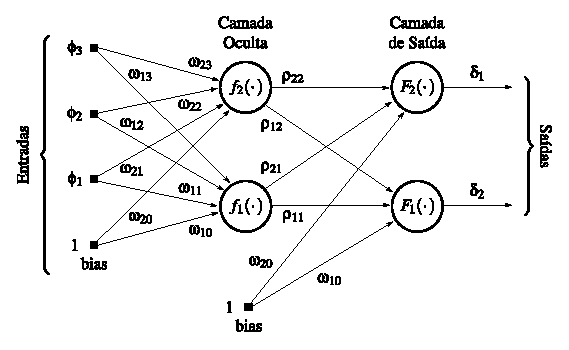
\includegraphics[width=0.65\textwidth]{imgs/rnas/eps/pmc}
    \caption{Diagrama esquemático de uma rede PMC.}
    \label{fig:pmc}
\end{figure}

\Glossary{PMC}{Perceptron de Múltiplas Camadas}
\Glossary{LMA}{Levenberg-Marquardt}

A opção pela estrutura de PMC se dá devido a sua simplicidade e capacidade de
aplicação em diversas áreas. Já a opção pelo treinamento com o algoritmo LMA
pode ser justificada por se tratar de um método Quase-Newton que acelera o
processo de convergência da rede, uma vez que leva em consideração termos de
ordens mais elevadas que o algoritmo {\it backpropagation}. 

Ademais, pode-se comentar que, apesar de ser possível realizar o treinamento das
redes através de uma linguagem de programação convencional, implementar tais
soluções, tão difundidas em {\it softwares} mundialmente reconhecidos como o
Matlab\reg\ e amplamente aceitas no meio acadêmico, está fora do escopo deste
trabalho.

Segundo \citeasnoun{norgaard:2000}, uma rede PMC básica possui seus neurônios
dispostos em camadas, recebendo como entrada as saídas dos neurônios da camada
imediatamente anterior ou, no caso da primeira camada, as entradas da rede. Por
possuir essa configuração essas redes são conhecidas como redes {\it
feedforward}.

Como mostrado na Fig. \ref{fig:pmc}, a segunda camada é conhecida como camada
de saída, pois produz as saídas da rede neral. A primeira camada é conhecida
como camada oculta ou intermediária por estar ``escondida'' entre as entradas da
rede ($\phi_1$, $\phi_2$ e $\phi_3$) e a camada de saída. Em
\citeasnoun{cybenko:1989} foi demonstrado que qualquer função contínua pode ser
aproximada por uma rede neural PMC que possua uma camada oculta com funções de
ativação sigmoidal ou tangente hiperbólica.

A Eq. \ref{eq:func_rede_pmc} expressa matematicamente o funcionamento de uma
rede neural PMC de duas camadas, como na Fig. \ref{fig:pmc}, em que $\delta_i$
representa a $i$-ésima saída da rede.

\begin{equation}\label{eq:func_rede_pmc}
\delta_i(t) = g_i[\phi,\theta] =
              F_i\colchete{\sum_{j=1}^{n_h}\rho_{i,j}f_j
              \parent{\sum_{l=1}^{n_\phi}\omega_{j,l}\phi_l+\omega_{j,0}}+
              \rho_{i,0}}
\end{equation}
\Glossary{$\delta_i$}{$i$-ésima saída da rede neural}
\Glossary{$\phi$}{Vetor de entradas da rede neural}
\Glossary{$\phi_l$}{$l$-ésima entrada da rede neural}
\Glossary{$\theta$}{Vetor de parâmetros ajustáveis da rede neural}
\Glossary{$F$, $f$}{Funções de ativação dos neurônios da rede neural}
\Glossary{$\rho$}{{\it biases}}
\Glossary{$\rho_{i,j}$}{{\it biases} que partem da camada $j$ e chegam na camada
                        $i$}
\Glossary{$\omega_{j,l}$}{Peso sináptico que parte do neurônio $l$ e chega no
                          neurônio $j$}
\Glossary{$n_h$}{Número de neurônios da camada oculta}
\Glossary{$n_\phi$}{Número de entradas da rede}

O vetor de parâmetros $\theta$ contém os pesos sinápticos e {\it biases}
($\omega_{j,l}$, $\rho_{i,j}$). O número de neurônios da camada oculta e o
número de entradas da rede são, respectivamente, $n_h$ e $n_\phi$, enquanto que
$F_i$ e $f_j$ são as funções de ativação dos neurônios das camadas de saída e
oculta, respectivamente. As funções de ativação mais comumente utilizadas são
mostradas nas equações \ref{eq:lin}, \ref{eq:sig} e \ref{eq:tan}.

\begin{equation}
\label{eq:lin}
f_l(x)=x \\
\end{equation} 

\Glossary{$f_l$}{Função de ativação linear}

\begin{equation}
\label{eq:sig}
f_s(x) = \frac{1}{1+e^{-x}}\\
\end{equation} 

\Glossary{$f_s$}{Função de ativação sigmoidal}

\begin{equation}
\label{eq:tan}
f_t(x) = \text{tanh}(x) = \frac{1-e^{-x}}{1+e^{-x}}\\
\end{equation}

\Glossary{$f_t$}{Função de ativação tangente hiperbólica}

% ------------------------------------------------------------------------------
\section{Identificação através de modelo neural}
\begin{comment}
Segundo \citeasnoun{reboucas:2009}, a realização de inferência utilizando RNAs
pode ser vista como um problema de identificação, uma vez que a rede neural
treinada deve ser capaz de representar, satisfatoriamente, a dinâmica existente
entre as variáveis secundárias e primárias do processo.
\end{comment}

Segundo \citeasnoun{reboucas:2009}, as estruturas de modelo baseadas em redes
neurais, apropriadas para a identificação de sistemas não-lineares, são
generalizações de modelos lineares.  Para \citeasnoun{lucena:2005}, essas
estruturas são caracterizadas por seu vetor de regressão, que nada mais é do que
um vetor que contém as variáveis utilizadas para estimar a saída do sistema.
Dependendo da escolha do vetor de regressão, diferentes estruturas de modelo
neural podem surgir. Estruturas FIR ({\it Finite Impulse Response}), ARX ({\it
AutoRegressive eXternal input}), ARMAX ({\it AutoRegressive Moving Average
eXternal input}), OE ({\it Output Error}) e SSIF ({\it State Space Innovations
Form}) são algumas das estruturas lineares mais conhecidas. Se o vetor de
regressão for selecionado para modelos ARX, a estrutura do modelo neural será
chamada NNARX ({\it Neural Network ARX}). Do mesmo modo, existirão também
modelos NNFIR, NNARMAX, NNOE e NNSSIF.

\Glossary{FIR}{{\it Finite Impulse Response}}
\Glossary{ARX}{{\it AutoRegressive eXogenous}}
\Glossary{ARMAX}{{\it AutoRegressive Moving Average eXogenous}}
\Glossary{OE}{{\it Output Error}}
\Glossary{SSIF}{{\it State Space Innovations Form}}
\Glossary{NNARX}{{\it Neural Network AutoRegressive eXogenous inputs}}
\Glossary{NNARMAX}{{\it Neural Network AutoRegressive Moving Average eXogenous
                        inputs}}
\Glossary{NNOE}{{\it Neural Network Output Error}}
\Glossary{NNSSIF}{{\it Neural Network State Space Innovations Form}}

Neste trabalho foi utilizado um modelo de rede baseado no NNARX descrito em
\citeasnoun{norgaard:2000}. A Fig. \ref{fig:nnarx} representa um esquema
simplificado do modelo adotado. A presença de regressores no modelo, relaciona a
saída da rede com seus valores passados de entrada e saída. A utilização desses
regressores é de fundamental importância para a identificação de sistemas.

\begin{figure}[htb]
\centering

\includegraphics[width=0.45\textwidth]{imgs/rnas/eps/nnarx}
\caption{Esquema de uma rede neural com estrutura NNARX.}
\label{fig:nnarx}
\end{figure}

\Glossary{$y$}{Saída da planta}
\Glossary{$u$}{Entrada da planta}
\Glossary{$d$}{Atraso de transporte}

A expressão matemática que descreve o modelo não-linear pode ser descrita
conforme Eq. \ref{eq:modelo_nnarx}.

\begin{equation}
\label{eq:modelo_nnarx}
\hat{y}(t) = g\parent{y(t-1), \ldots, y(t-n), u(t-d), \ldots, u(t-d-m)}
\end{equation}

\Glossary{$\widehat{y}(t)$}{Saída estimada pela rede neural}
\Glossary{$n$}{Ordem de saída}
\Glossary{$m$}{Ordem de entrada}

Nessa equação $\hat{y}$ representa a saída estimada, $d$ o atraso de transporte,
$n$ a ordem da saída, $m$ a ordem de entrada da planta, $g( \cdotp )$ uma função
não linear mapeada pela rede neural, $y$ a saída da planta e $u$ a entrada da
planta.

A estimativa gerada pela estrutura NNARX é sempre estável, uma vez que
representa relações puramente algébricas entre a estimativa e as medições
passadas de entradas e saídas do processos, não existindo a realimentação da
saída estimada.

% ------------------------------------------------------------------------------
\subsection{Determinação da ordem do modelo}
\label{sec:det_ordem}
Em sistemas de identificação {\it blackbox}\footnote{Também conhecida como
identificação em caixa-preta, a identificação {\it blackbox} pressupõe que não
se dispõe de nenhuma informação sobre a estrutura interna ou sobre o
funcionamento do sistema. Nesse tipo de abordagem, faz-se uso de uma análise da
relação dos valores de saída obtidos a partir dos estímulos fornecidos nas
entradas do sistema.}, como o utilizado neste trabalho, é de fundamental
importância que a ordem do modelo seja determinada adequadamente.  Uma escolha
inadequada poderá fazer com que a dinâmica do processo não seja assimilada pela
rede neural, fazendo com que as estimativas geradas possuam erro médio
consideravelmente alto. Segundo \citeasnoun{arruda:2003}, existe uma ordem de
modelo ótima que permite obter o menor erro entre o modelo estimado e o sistema
real.

A ordem de entrada ($m$) e de saída ($n$) de um sistema desse tipo pode ser
obtida a partir da realização de testes ou simulações com o processo. Por
facilidade de representação, considerar-se-á a ordem de entrada igual a ordem de
saída ($m = n$). No capítulo \ref{cap:resultados} poderão ser vistos alguns
resultados dos testes que foram realizados para a determinação da ordem das
redes de identificação e de detecção e diagnóstico de falhas.

% ------------------------------------------------------------------------------
\subsection{Seleção do modelo}
Existem diversas estruturas de modelagem, cada uma com suas vantagens e
desvantagens. Segundo \citeasnoun{norgaard:2000}, o problema da seleção das
estruturas pode ser dividido em duas partes. A primeira delas é a parte da
seleção da ``família'' de estruturas de modelagem. Dependendo do sistema, as
estruturas podem ser: modelos lineares, redes PMC, redes de função de base
radial, {\it wavelets} etc. Já a segunda, é a parte da seleção do subconjunto da
família escolhida.

A escolha por uma estrutura do tipo NNARX se deu pelas diversas vantagens em se
utilizar RNAs para estimar valores e por se tratar de um modelo que não faz uso
de realimentação da saída estimada, o que permite dizer que este é estável no
sentido BIBO\footnote{Um sistema é dito BIBO estável quando, para qualquer
entrada limitada, obtém-se uma saída também limitada.} ({\it Bounded Input,
Bounded Output}). Para \citeasnoun{norgaard:2000}, devido a estas
características, o modelo NNARX é um dos mais utilizados quando o sistema a ser
modelado é determinístico ou o nível de ruído não é significativo.

\Glossary{BIBO}{\it Bounded Input, Bounded Output}

De maneira resumida, após a seleção da estrutura, segue-se uma sequência de
etapas até que o modelo possa representar adequadamente o sistema, de acordo com
algum critério específico, como por exemplo, o erro médio quadrático (EMQ) de
estimativa, que é calculado a partir da Eq. \ref{eq:emq} e utilizado no
algoritmo de treinamento da RNA para determinar o ponto de parada (fim do
treinamento).

\Glossary{EMQ}{Erro Médio Quadrático}

\begin{equation}\label{eq:emq}
\text{EMQ} = \sqrt{\frac{1}{N}
             \sum_{i=1}^{N}\pfrac{y_i - \widehat{y_i}}{y_i}^2}
\end{equation}

Nessa equação, $N$ representa o número de amostras de validação, $y_i$ o valor
real e $\widehat{y_i}$ o valor estimado.

\Glossary{$N$}{Número de amostras de validação}
\Glossary{$y_i$}{$i$-ésimo valor real de saída da planta}
\Glossary{$\widehat{y_i}$}{$i$-ésimo valor estimado pelo sistema}

Tendo conhecido as características das redes neurais que serão utilizadas no
desenvolvimento deste trabalho, o capítulo seguinte trará os principais
conceitos e terminologias relacionadas ao tema de detecção e diagnóstico de
falhas.

\mychapter{Detecção e diagnóstico de falhas}
\label{cap:detec_diag}

Com a demanda cada vez mais crescente com relação a eficiência, a qualidade dos
produtos e integração dos processos no setor industrial, aliada aos altos custos
envolvidos e as mais diversas necessidades de segurança, torna-se claro a
importância dos sistemas de supervisão e dos sistemas de DDF
\cite{isermann:2006}.

Atualmente, devido ao nível de complexidade envolvido em um processo industrial,
os sistemas de supervisão e proteção exigem as mais avançadas técnicas
oferecidas pela engenharia moderna e, ainda assim, demandam um esforço contínuo
por parte dos pesquisadores e engenheiros para que sejam desenvolvidas novas
tecnologias que venham a suprir essa necessidade \cite{silva:2008}.

Considerando tais aspectos, este capítulo mostrará os conceitos relacionados ao
desenvolvimento de um sistema de DDF que fará uso de RNAs. Inicialmente, serão
mostrados os principais conceitos e terminologias utilizadas na área, destacando
alguns métodos de DDF. Ao final do capítulo serão expostas as técnicas de DDF
que fazem uso de RNAs.

% ------------------------------------------------------------------------------
\section{Conceitos e terminologias}\label{sec:propriedades}
Segundo \citeasnoun{kaanich:2002}, os sistemas computacionais podem ser
caracterizados por cinco propriedades fundamentais: funcionalidade, usabilidade,
desempenho, custo e {\it dependabilidade}. Para \citeasnoun{laprie:1992}, o
termo {\it dependabilidade}, que nada mais é do que a tradução literal do termo
inglês {\it dependability}, está relacionado com a capacidade de um sistema
prestar um serviço que possa ser, justificadamente, confiável. O serviço
prestado se refere ao comportamento do sistema percebido por seus usuários, os
quais também serão sistemas (máquinas físicas ou seres humanos), que interagem
com o anterior.

De acordo com \citeasnoun{laprie:1994}, dependendo das aplicações envolvidas, o
termo dependabilidade pode ainda ser visto de acordo com suas diferentes, mas
complementares, propriedades:

\begin{itemize}
    \item {\bf Disponibilidade:} Prontidão para o uso;
    \item {\bf Confiabilidade:} Continuidade do serviço;
    \item \textbf{Proteção (\textit{safety}):} Não ocorrência de consequências
          catastróficas para o meio;
    \item {\bf Confidencialidade:} Não ocorrência da divulgação não-autorizada
          da informação;
    \item {\bf Integridade:} Não ocorrência de alterações indevidas da
          informação;
    \item {\bf Manutenção:} Aptidão para sofrer reparos e evolução.
\end{itemize}

A associação da integridade com a disponibilidade e a confidencialidade leva à
\textbf{Segurança (\textit{security})}.

Apesar do termo dependabilidade ser utilizado na maioria das vezes dessa forma,
o dicionário Michaelis, traduz tal termo como {\it confiabilidade} ou {\it
garantia de funcionamento}. Assim sendo, daqui para frente, utilizar-se-á a
palavra {\it confiável}, ou suas variações linguísticas, para se referir ao
termo {\it dependable}. Quando for desejado fazer referência a propriedade da
confiabilidade de um sistema, tal intenção será claramente especificada pelo
texto.

% ------------------------------------------------------------------------------
\section{Sistemática da dependabilidade}
\citeasnoun{avizienis:2000} e \citeasnoun{kaanich:2002} mostram que para se
desenvolver um Sistema Computacional Confiável (SCC, do inglês {\it Dependable
Computing System -- DCS}), faz-se uso de diferentes técnicas, tais como as
técnicas de: {\bf prevenção}, {\bf tolerância}, {\bf supressão} e {\bf previsão}
de falhas.

O estudo sobre a {\it prevenção} de falhas envolve a seleção de metologias de
projeto e de tecnologias adequadas para a escolha e a aplicação dos componentes
no sistema, ou seja, busca não introduzir ou evitar que aconteçam falhas. A {\it
tolerância} a falhas está mais relacionada com a continuidade da prestação do
serviço quando uma falha vier a ocorrer. Algumas das técnicas mais conhecidas
são: mascaramento de falhas, redundância de dispositivos/sistemas e a
detecção/recuperação de falhas. A {\it supressão} das falhas procura minimizar
as consequências relativas à presença de uma falha através de mecanismos de
verificação, diagnóstico e correção. A {\it previsão} de falhas está relacionada
com a estimativa que pode ser feita sobre a presença, a criação e a consequência
que as falhas venham a causar no sistema. Para isso, faz uso de critérios
avaliativos, técnicas de injeção de falhas e testes de resistência.

Além dessas técnicas, é válido também fazer referência aos termos {\bf avaria},
{\bf erro} e {\bf falha}, conceitualmente abordados de diferentes maneiras por
vários autores. Os conceitos relativos a essa nomenclatura serão melhor
explicados na seção \ref{sec:avaria_erro_falha}.

\begin{comment}
\begin{itemize}
    \item {\bf Técnicas de prevenção:} Como prevenir a ocorrência ou a introdução de
          falhas;
    \item {\bf Técnicas de tolerância:} Como oferecer um serviço ``correto'' na
          presença de falhas;
    \item {\bf Técnicas de supressão:} Como reduzir o número ou atenuar a
          gravidade das falhas;
    \item {\bf Técnicas de previsão:} Como estimar o número atual, a incidência
          futura e as consequências das prováveis falhas.
\end{itemize}
\end{comment}

A partir dessas informações, \citeasnoun{avizienis:2000} separa os termos acima
relacionados em três grupos: os atributos (propriedades), as ameaças e os meios
pelos quais a dependabilidade é atingida. Tal divisão pode ser observada na Fig.
\ref{fig:div_avizienis}.

\begin{figure}[htb]
\centering
\footnotesize
\[
\text{Dependabilidade}
\left\{
\begin{array}{l}
\text{Atributos}
    \left\{
    \begin{array}{l}
        \text{Disponibilidade}\\
        \text{Confiabilidade}\\
        \text{Proteção}\\
        \text{Confidencialidade}\\
        \text{Integridade}\\
        \text{Manutenção}\\
        \text{Segurança}
    \end{array}
    \right.
\\
\\
\text{Ameaças}
    \left\{
    \begin{array}{l}
        \text{Avaria}\\
        \text{Erro}\\
        \text{Falha}
    \end{array}
    \right.
\\
\\
\text{Meios}
    \left\{
    \begin{array}{l}
        \text{Prevenção}\\
        \text{Tolerância}\\
        \text{Supressão}\\
        \text{Previsão}
    \end{array}
    \right.
\end{array}
\right.
\]
\caption{Classificação sistemática da dependabilidade.}
\label{fig:div_avizienis}
\end{figure}

O primeiro grupo, cujos elementos foram brevemente explicados na seção
\ref{sec:propriedades}, permite expressar as propriedades esperadas e analisar a
qualidade de um sistema confiável. Já o segundo grupo traz os termos utilizados
para expressar características indesejadas -- mas em princípio não inesperadas
-- que causa ou fazem com que um sistema passe a ser não-confiável. Por fim, o
terceiro grupo exibe os meios ou as técnicas pelas quais torna-se possível
oferecer um serviço confiável.

% ------------------------------------------------------------------------------
\section{Avarias, erros e falhas}\label{sec:avaria_erro_falha}
Em um processo real, todos os recursos utilizados, sejam físicos ou
implementados em {\it software}, estão sujeitos a interrupções ou a
comprometimentos operacionais.

Em sistemas críticos, tais como as aeronaves ou as usinas nucleares, essas
situações fazem com que pequenos ``deslizes operacionais'' venham a trazer
grandes e indesejáveis consequências. Dentre diversos outros exemplos, pode-se
destacar o acidente do {\it Airbus 320} da TAM em 2007, que não conseguiu parar
ao aterrissar no aeroporto de Congonhas, São Paulo, no qual morreram 199 pessoas
(12 em solo e 187 no avião) e o desastre da usina nuclear de Chernobil, que
liberou cerca de 400 vezes mais contaminação do que a bomba nuclear que foi
lançada em de Hiroshima.

Esses exemplos fazem-nos refletir sobre como os sistemas de controle podem
evoluir para evitar que catástrofes ainda maiores venham a ocorrer. Ou seja,
como as propriedades de um sistema de controle confiável poderão ser mantidas
mesmo na presença de avarias, erros e falhas no processo.

Segundo \citeasnoun{nelio:2002}, apesar do termo falha ser utilizado, em muitos
dos casos, como um termo vago, abrangendo também o significado de avarias e
erros, existe uma diferença entre esses conceitos que deve ser destacada.

O termo {\bf avaria} ({\it failure}) deve ser utilizado para indicar que houve
um desvio do comportamento no sistema, o que o torna incapaz de fornecer o
serviço para o qual foi designado. Um {\bf erro} ({\it error}), entretanto, está
relacionado com estado do sistema e pode levar a uma avaria. De maneira
resumida, se há um erro no estado do sistema, então existe uma sequência de
ações que podem ser executadas e que levarão a avarias, a não ser que medidas de
correção venham a ser tomadas. Por fim, mas não menos importante, o termo {\bf
falha} ({\it fault}) é a causa de um erro e está associado à noção de defeitos.
Normalmente, diz-se que falha pode ser definida como sendo um defeito que possui
o potencial de gerar erros \cite{nelio:2002,weber:2002}.

Alguns autores nacionais costumam traduzir os termos {\it failure} como falha e
{\it fault} como falta. Entretanto, costuma-se falar em sistemas de controle
tolerante a ``falhas'' e não em sistemas de controle tolerantes a ``faltas''.
Observa-se então a necessidade de um maior cuidado com relação a utilização
dessas palavras, pois as avarias ({\it failures}) não podem ser toleradas.

\begin{comment}
Por esse motivo, ao longo do texto, quando for necessário se referir ao termo
{\it failure}, será utilizada a palavra avaria. Já o termo falha será utilizado
de maneira mais abrangente, envolvendo os conceitos de erro e de falha
explicados anteriormente.
\end{comment}

Como em muitos dos casos os sistemas são compostos de subsistemas, é comum se
observar que uma falha leva a um erro que por sua vez pode levar a uma avaria,
que gera novas falhas e dá início a uma reação em cadeia, tal como a Fig.
\ref{fig:reacao_cadeia}. Contudo, nem sempre uma falha conduz a um erro, assim
como nem sempre um erro conduz a uma avaria, mas todos os erros resultam de
falhas e todas as avarias resultam de erros.

\begin{figure}[htb]
\centering
\[
\ldots
\quad\Longrightarrow\quad
\text{Falha} 
\quad\longrightarrow\quad
\text{Erro}
\quad\longrightarrow\quad
\text{Avaria}
\quad\Longrightarrow\quad
\text{Falha}
\quad\longrightarrow\quad
\ldots
\]
    \caption{Reação em cadeia das falhas, erros e avarias.}
    \label{fig:reacao_cadeia}
\end{figure}

Uma outra maneira de visualizar a diferença existente entre cada um desses
termos pode ser observada na Fig. \ref{fig:mapa_conceitos}.

\begin{figure}[htb]
\centering
    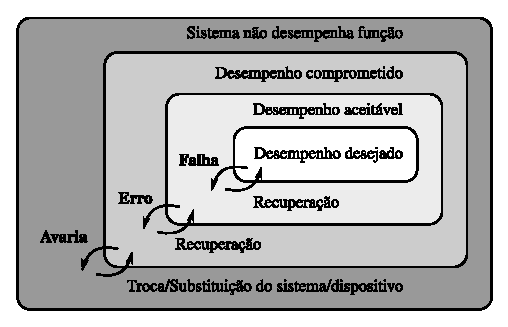
\includegraphics[width=0.5\textwidth]{imgs/detec_diag/eps/mapa_conceitos}
    \caption{Mapa de conceitos relacionados a avarias, erros e falhas em um
             sistema.}
    \label{fig:mapa_conceitos}
\end{figure}

\citeasnoun{weber:2002} afirma ainda que as falhas são inevitáveis, uma vez que
os componentes físicos do sistema envelhecem e estão sempre sujeitos as
interferências externas, ambientais ou humanas. Mostra também que, assim como os
sistemas físicos, os {\it softwares} também são vítimas, pois estão a mercê da
alta complexidade dos processos e da fragilidade humana em trabalhar com grande
volume de detalhes de especificação/operação.

% ------------------------------------------------------------------------------
\subsection{Tipos de falhas}

\begin{comment}
\citeasnoun{laprie:1994} mostra que existem cinco classes elementares para as
falhas, conforme Fig. \ref{fig:class_laprie}.

\begin{figure}[htb]
\centering
\footnotesize
\[
\text{Falha}
\left\{
\begin{array}{l}
\text{Causas fenomenológicas}
    \left\{
    \begin{array}{l}
        \text{Falhas físicas}\\
        \text{Falhas humanas}
    \end{array}
    \right.
\\
\\
\text{Natureza}
    \left\{
    \begin{array}{l}
        \text{Falhas acidentais}\\
        \text{Falhas intencionais, não-maliciosas}\\
        \text{Falhas intencionais, maliciosas}
    \end{array}
    \right.
\\
\\
\text{Criação/Ocorrência}
    \left\{
    \begin{array}{l}
        \text{Falhas de desenvolvimento}\\
        \text{Falhas operacionais}
    \end{array}
    \right.
\\
\\
\text{Limitações do sistema}
    \left\{
    \begin{array}{l}
        \text{Falhas internas}\\
        \text{Falhas externas}
    \end{array}
    \right.
\\
\\
\text{Persistência}
    \left\{
    \begin{array}{l}
        \text{Falhas permanentes}\\
        \text{Falhas temporárias}
    \end{array}
    \right.
\end{array}
\right.
\]
    \caption{As cinco classes elementares das falhas.}
    \label{fig:class_laprie}
\end{figure}

\end{comment}

De acordo com \citeasnoun{silva:2008}, as falhas em um processo industrial podem
ser classificadas em relação a vários aspectos. Em se tratando da classificação
quanto ao tempo, as falhas podem ser abruptas, incipientes ou intermitentes, tal
como mostra a Fig. \ref{fig:tipos_falha}.

\begin{figure}[H]
\centering
    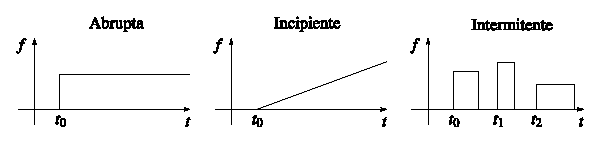
\includegraphics[width=0.75\textwidth]{imgs/detec_diag/eps/tipos_falha}
    \caption{Características temporais das falhas quanto a sua persistência.}
    \label{fig:tipos_falha}
\end{figure}

\begin{comment}
De acordo com essa classificação, percebe-se que não existirá um sistema
que venha a falhar somente uma vez. Por mais que as falhas demorem a acontecer,
elas são inevitáveis.
\end{comment}

As {\it falhas abruptas} surgem repentinamente, podendo ser decorrentes de
imprevistos ou até mesmo de acidentes. Essas falhas mudam o comportamento do
processo rapidamente, exigindo contra-ações velozes e eficazes que possam
minimizar as consequências do ocorrido.

As {\it falhas incipientes} iniciam a partir de pequenos desvios comportamentais
do sistema, podendo ser mascaradas pelos controladores.  Muitas vezes essas
falhas acabam passando despercebidas pelos operadores ou até mesmo pelos
sistemas de detecção e diagnóstico de falhas.

As {\it falhas intermitentes} são aquelas que ocorrem durante um certo período
de tempo e, em seguida, desaparecem, voltando a aparecer após um novo intervalo.
Podem ser causadas por alguma perturbação periódica ou por alguma situação que
se repita ciclicamente.

Considerando a localização das falhas, estas podem ocorrer nos sensores, nos
atuadores ou na estrutura do sistema \cite{silva:2008}. As {\it falhas nos
sensores} podem ser observadas através de variações específicas nas medições, as
quais podem ser descaracterizadas como variações válidas do sistema. As {\it
falhas nos atuadores} podem ser vistas como qualquer mau funcionamento do
equipamento que atua no sistema. As {\it falhas na estrutura}, ou {\it falhas
estruturais}, ocorrem quando alguma alteração do sistema muda, de alguma forma,
a relação original de entrada e saída do processo ou quando ocorre algum
problema com algum dos dispositivos, desde que não sejam sensores ou atuadores,
como por exemplo, os transmissores de sinal.

Considerando então um processo genérico, pode-se citar como exemplos de falhas
aquelas exibidas pela Tab. \ref{tab:falhas}.

\begin{table}[htb]
\centering
\caption{Exemplos de falhas para um processo genérico.}
\label{tab:falhas}
\vspace{0.25cm}
\begin{tabular}{|c|c|c|}
\hline
{\bf Sensores} & {\bf Atuadores} & {\bf Estrutura}\\
\hline
\hline
Erro de leitura & Erro de escrita & Erro de transmissão\\
\hline
Descalibramento & Erro de leitura & Perda de comunicação\\
\hline
Sensibilidade à ruído & Sensibilidade à ruído & Sensibilidade a ruído
(transmissor)\\
\hline
Queima & Queima & Queima (transmissor)\\
\hline
- & Atraso de transporte & Atraso de propagação de sinais\\
\hline
\end{tabular}
\end{table}

Maiores detalhes sobre as propriedades e a classificação das falhas podem ser
encontradas em \citeasnoun{laprie:1992}, \citeasnoun{laprie:1994},
\citeasnoun{weber:2002} e \citeasnoun{isermann:2006}.

% ------------------------------------------------------------------------------
%\section{Os meios para se atingir a dependabilidade}
%\label{sec:tecnicas}

% ------------------------------------------------------------------------------
\section{Detecção e diagnóstico de falhas}
Segundo \citeasnoun{chiang:2001}, detectar, diagnosticar e ``remover'' uma falha
é uma das formas de se garantir que as operações de um processo satisfaçam as
especificações de desempenho. Essas ações estão associadas com a noção de
supervisão e monitoramento de processos.

Para eles, supervisionar e monitorar determinado processo tem por objetivo
garantir o sucesso das operações planejadas e reconhecer as anomalias
comportamentais. A informação a ser disponibilizada por um sistema de
monitoramento não deve, tão somente, informar ao operador do sistema sobre o que
está acontecendo, mas auxiliá-lo a tomar medidas corretivas com o intuito de
sanar o problema. Como resultado disso, o tempo em que o sistema estará
inoperante será reduzido, a proteção do sistema aumentará e os custos
relacionados diminuirão.

Uma vez que os processos industrias estão se tornando cada vez mais integrados e
complexos, a ocorrência de falhas também passa a ser um fator de complicação. As
falhas que antes poderiam ser detectadas facilmente por medições diretas de
determinada variável passam a depender de um conjunto de variáveis que atuam
simultaneamente. Além disso, se uma falha é detectada em um determinado ponto de
um sistema sistema, a causa do problema pode estar próxima ou distante,
dependendo do grau de complexidade envolvido. Como exemplo, uma simples falha em
uma aeronave pode causar indicações de falha em diversos subsistemas de
segurança \cite{vach:2006}.

Para \citeasnoun{chiang:2001}, existem quatro fases envolvidos no monitoramento
de processos: {\bf detecção}, {\bf isolamento}, {\bf diagnóstico} e {\bf
recuperação} de falhas, conforme mostrado pela Fig.
\ref{fig:fases_monitoramento}.

\begin{figure}[htb]
\centering
    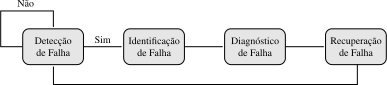
\includegraphics[width=0.65\textwidth]
                    {imgs/detec_diag/eps/fases_monitoramento}
    \caption{Fases envolvidas no monitoramento de processos.}
    \label{fig:fases_monitoramento}
\end{figure}

A {\it detecção da falha} consiste em determinar se ocorreu ou não uma falha. A
detecção antecipada ou precoce pode fornecer informações valiosas quanto aos
problemas que venham a surgir. Através de ações apropriadas, pode-se evitar
perturbações graves ao processo.

A {\it identificação da falha} tem por objetivo identificar as variáveis mais
importantes para que se realize um diagnóstico apropriado. Para isso, essa fase
procura concentrar as atenções do operador nos subsistemas mais pertinentes à
falha, de tal modo que o efeito desta possa ser eliminado de maneira mais
eficiente.

A fase de {\it diagnóstico da falha} determina que falha ocorreu. De acordo com
\citeasnoun{isermann:2004}, essa fase deverá indicar o maior número de detalhes
possíveis a respeito da falha, tais como a intensidade, a localização e o
momento em que a falha foi detectada. Essa fase é considerada essencial para uma
contra-ação ou eliminação da falha.

A fase de {\it recuperação da falha}, também conhecida como fase de {\it
intervenção}, tem por objetivo remover o efeito da falha para com o sistema,
dando início a um novo ciclo de detecção e diagnóstico.

Apesar de estarem explicitamente colocados como uma sequência de ações, nem
sempre todas as fases são estritamente necessárias necessárias
\cite{chiang:2001}. 

Para \citeasnoun{venkatasu:2003a}, a automatização das formas de detecção e
diagnóstico compõe o primeiro passo de um sistema de gestão de eventos anormais
Ao longo de vários anos, muitas soluções vem sendo desenvolvidas e um grande
número de técnicas já foram utilizadas. Exemplos dessas técnicas são as árvores
de falhas, os digrafos, as abordagens analíticas, os sistemas especialistas e as
RNAs.

\fussy
Do ponto de vista de modelagem, existem métodos que exigem grande precisão com
relação ao modelo de processo, outros que exigem modelos semi-quantitativos ou
ainda modelos qualitativos. Por outro lado, existem métodos que não necessitam
de nenhuma informação do modelo, utilizando somente informações do histórico do
processo \cite{venkatasu:2003a}.
\sloppy

Conforme mostrado no Capítulo \ref{cap:introducao}, a classificação dos métodos
de DDF pode variar de autor para autor
\cite{venkatasu:2003a,angeli:2004,zhang:2008,isermann:2006}. A abordagem aqui
escolhida irá considerar a classificação adotada em \citeasnoun{isermann:2006},
até então considerada a mais intuitiva.

% ------------------------------------------------------------------------------
\section{Métodos de detecção}
Nas seções seguintes será feita uma breve análise dos métodos de detecção de
falhas abordados em \citeasnoun{isermann:2006}. Vale salientar que existem, na
literatura, vários outros métodos de detecção de falhas. Deseja-se aqui trazer
alguns exemplos.

% ------------------------------------------------------------------------------
\subsection{Detecção de falhas com verificação de limites}
Considerado como um dos métodos mais simples e intuitivos, a detecção de falhas
com verificação de limites baseia-se na medição direta de uma determinada
variável e a comparação de seu valor absoluto ou de sua tendência com um
limítrofe previamente especificado.

A verificação de valores absolutos, estabelece que dois limiares ou limítrofes
fixos são estabelecidos: $Y_{max}$ e $Y_{min}$. O funcionamento normal do
sistema consiste em verificar se a variável $Y$ está ou não contida nesse
intervalo:

\begin{equation}
Y_{min} < Y < Y_{max}
\end{equation}

Essa abordagem considera que o processo está funcionando normalmente quando a
variável monitorada encontra-se dentro de uma zona de tolerância. Quando a
variável monitorada excede um dos limiares estabelecidos, deduz-se que haverá
uma falha em algum ponto do processo.

Por mais simples que pareça, este método é aplicado na maioria dos sistemas de
automação, tais como: verificação da pressão mínima em oleodutos, da temperatura
máxima em sistemas de refrigeração de motores, a pressão mínima de circulação de
gás em refrigeradores.

Uma outra abordagem utiliza a verificação de tendência da variável medida. Um
exemplo simples faz uso da primeira derivada da variável $\dot{Y} = dY(t)/dt$ e
verifica se esta tendência está ou não dentro de uma faixa pré-estabelecida:

\begin{equation}
\dot{Y}_{min} < \dot{Y} < \dot{Y}_{max}
\end{equation}

Exemplos dessas duas abordagens podem ser observados na Fig.
\ref{fig:detec_ver_lim}.

\begin{figure}[htb]
\centering
    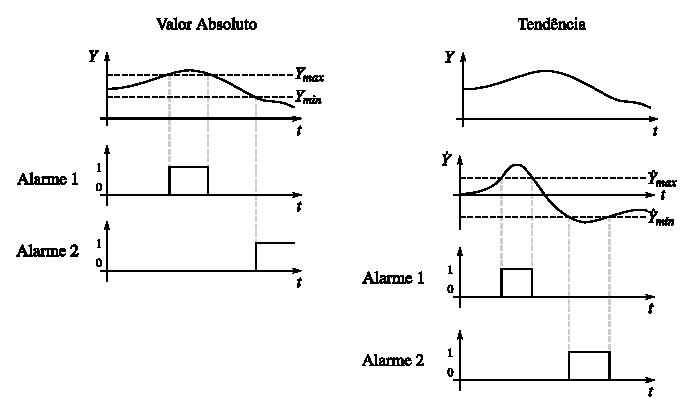
\includegraphics[width=0.85\textwidth]{imgs/detec_diag/eps/detec_ver_lim}
    \caption{Exemplo de detecção com verificação de limites.}
    \label{fig:detec_ver_lim}
\end{figure}

% ------------------------------------------------------------------------------
\subsection{Detecção de falhas com modelos de sinais}
Diversos sinais medidos em um processo apresentam oscilações de natureza
harmônica ou estocástica. Se as mudanças nesse sinal estiverem relacionadas com
as falhas nos sensores, atuadores ou ainda com as falhas estruturais, uma
maneira de se detectar essas falhas é o de se utilizar métodos de detecção
baseados em modelos de sinais.

Na Fig. \ref{fig:detec_mod_sin} é exibido um diagrama esquemático que resume os
princípios da detecção de falhas com modelos de sinais.

\begin{figure}[htb]
\centering
    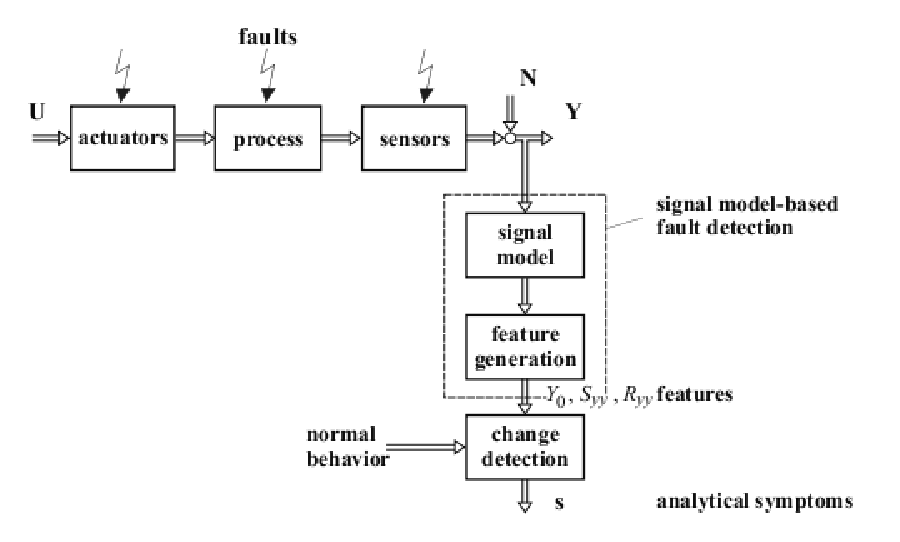
\includegraphics[width=0.75\textwidth]{imgs/detec_diag/eps/detec_mod_sin}
    \caption{Diagrama esquemático da detecção de falhas com modelos de sinais.}
    \label{fig:detec_mod_sin}
\end{figure}

De maneira resumida pode-se dizer que as características do sinal medido, tais
como amplitude, fase, espectro de frequências, dentre outras, são calculadas a
partir de modelos matemáticos do sinal e comparadas com as características
observadas durante o funcionamento normal. As diferenças comportamentais geradas
pela comparação, denominadas de {\it sintomas analíticos}, são utilizadas para
realizar a detecção das falhas.

% ------------------------------------------------------------------------------
\subsection{Detecção de falhas com observadores e estimadores de estado}

% ------------------------------------------------------------------------------
\subsection{Detecção de falhas com equações de paridade}

% ------------------------------------------------------------------------------
\subsection{Detecção de falhas com métodos de identificação}

% ------------------------------------------------------------------------------
\section{Métodos de diagnóstico}

% ------------------------------------------------------------------------------
\subsection{diagnóstico de falhas com métodos de classificação}

% ------------------------------------------------------------------------------
\subsection{diagnóstico de falhas com métodos de inferência}

% ------------------------------------------------------------------------------
\section{Detecção e diagnóstico de falhas com RNAs}

Com a introdução das novas tecnologias de medição e o consequente aumento do
número de instrumentos nos processos industrias, as informações e os dados
disponíveis da operação do sistema passam a ser essenciais para as atividades de
supervisão e controle. Como exemplo, diversas estratégias de detecção e
diagnóstico de falhas fazem uso do histórico do processo ........ dentre essas
estratégias... RNAs


\mychapter{Sistema proposto}
\label{cap:sistema}

Uma vez que se abordou o conhecimento teórico relativo ao sistema proposto ao
longo dos capítulos anteriores, pode-se agora mostrar como esse sistema será
constituído.

Assim sendo, a primeira parte do capítulo descreverá em detalhes o modelo de
estudo de caso escolhido para ser simulado, mostrando suas características e
limitações. Em seguida a atenção será voltada para as estruturas neurais de
identificação do modelo e de detecção das falhas, mostrando ao final como serão
realizadas as simulações.

% ------------------------------------------------------------------------------
\section{Estudo de caso}
Ao final do Cap. \ref{cap:introducao}, após ter-se comentado sobre a utilização
das RNAs em sistemas de DDF, propôs-se que será desenvolvido um sistema para
realizar a detecçao e o diagnóstico de falhas em um processo dinâmico. Para que
isso seja possível serão utilizadas estruturas neurais que farão uso de
determinados valores obtidos a partir das medições realizadas no processo.

O processo em questão, ao qual se refere o parágrafo anterior, é formado por um
sistema de tanques acoplados desenvolvidos pela Quanser\reg, representado
esquematicamente na Fig. \ref{fig:tanques}.

\begin{figure}[htb]
\centering
    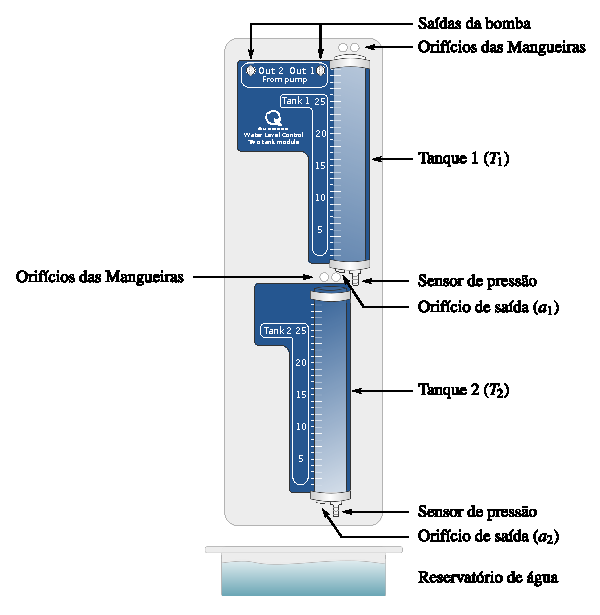
\includegraphics[width=0.7\textwidth]{imgs/sistema/eps/tanques}
    \caption{Sistema de tanques acoplados da Quanser\reg.}
    \label{fig:tanques}
\end{figure}

O sistema original consiste de uma bomba de água de corrente contínua e dois
tanques acoplados. A alimentação de água pela bomba se dá de forma vertical
através de dois orifícios com conectores normalmente fechados, de diferentes
diâmetros, denominados {\it Out 1} e {\it Out 2}. Para facilitar o entendimento
e evitar confusões com relação aos orifícios de saída dos tanques ($a_1$ e
$a_2$), esses orifícios serão tratados como orifícios de entrada.

\Glossary{$a_i$}{Orifício de saída $i$}

Os tanques ($T_1$ e $T_2$) são montados na parte frontal do suporte de base e
posicionados de tal forma que a água flui do tanque superior ($T_1$) para o
tanque inferior ($T_2$) através do orifício $a_1$, e do tanque inferior para o
reservatório através do orifício $a_2$. As vazões de saída dos tanques variam de
acordo com a mudança desses orifícios, disponibilizados em três diâmetros
diferentes pelo fabricante.

\Glossary{$T_1$}{Tanque superior}
\Glossary{$T_2$}{Tanque inferior}

Além dos diferentes orifícios de saída, o fabricante também disponibiliza um
conjunto de mangueiras, tornando possível a utilização dos dois orifícios de
entrada, bombeando água para os dois tanques simultaneamente. As dimensões de
cada um dos orifícios e os demais parâmetros do sistema podem ser visualizadas
na Tab. \ref{tab:dimensoes}.

\begin{table}[!htb]
\centering
\caption{Dimensões e parâmetros do sistema de tanques.}
\label{tab:dimensoes}
\vspace{0.25cm}
\begin{tabular}{|l|c|c|c|}
\hline
{\bf Nome} & {\bf Símbolo} & {\bf Valor} & {\bf Unidade}\\
\hline
\hline
\multicolumn{4}{|l|}{{\bf Bomba}}\\
\hline
\hline
Constante de fluxo & $K_m$ & 4,6 & (cm${}^3$/s)/V\\
\hline
Limites de Tensão & $V_{p_{\text{\tiny MIN/MAX}}}$ & $\pm 15$ & Volts\\
\hline
Orifício de entrada 1 & {\it Out 1} & 0,635 & cm\\
\hline
Orifício de entrada 2 & {\it Out 2} & 0,4763 & cm\\
\hline
\multicolumn{4}{|l|}{{\bf Tanque 1/Tanque 2}}\\
\hline
\hline
Altura & $H_1$/$H_2$ & 30 & cm\\
\hline
Diâmetro interno & -- & 4,445 & cm\\
\hline
Área de secção transversal & $A_1$/$A_2$ & 15,517916547 & cm${}^2$\\
\hline
Sensibilidade do sensor & -- & 5 & cm/V \\
\hline
\multicolumn{4}{|l|}{{\bf Orifícios de saída -- Diâmetros}}\\
\hline
\hline
Orifício pequeno & $a_{i_{\text{\tiny PEQ}}}$ & 0,3175 & cm\\
\hline
Orifício médio & $a_{i_{\text{\tiny MED}}}$ & 0,47625 & cm\\
\hline
Orifício grande & $a_{i_{\text{\tiny GDE}}}$ & 0,555625 & cm\\
\hline
\multicolumn{4}{|l|}{{\bf Orifícios de saída -- Áreas}}\\
\hline
\hline
Orifício pequeno & $a_{i_{\text{\tiny PEQ}}}$ & 0,079173044 & cm${}^2$\\
\hline
Orifício médio & $a_{i_{\text{\tiny MED}}}$ & 0,178139348 & cm${}^2$\\
\hline
Orifício grande & $a_{i_{\text{\tiny GDE}}}$ & 0,242467446 & cm${}^2$\\
\hline
\multicolumn{4}{|l|}{{\bf Sensores}}\\
\hline
\hline
{\it Range} de pressão & -- & 0 - 1 & PSI\\
\hline
{\it Range} de nível & -- & 0 - 30 & cm\\
\hline
Constante de sensibilidade & $K_s$ & $6,25\times$ & cm/V\\
\hline
\end{tabular}
\end{table}

Dentre as várias combinações possíveis obtidas a partir da mudança dos orifícios
de entrada e saída, as três configurações sugeridas pelo manual do fabricante
encontram-se representadas na Fig. \ref{fig:config_fab}. Cada uma dessas
configurações modifica a dinâmica do processo, permitindo que sejam projetados e
analisados diferentes tipos de controladores.

\begin{figure}[!htb]
\centering
\subfigure[Configuração 1]
{
    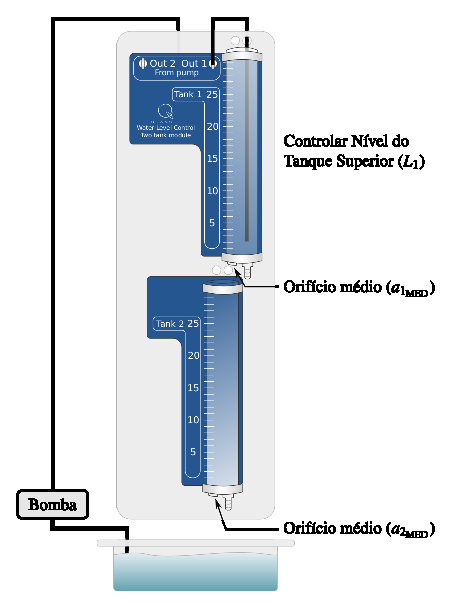
\includegraphics[width=0.31\textwidth]{imgs/sistema/eps/config_fab_1}
    \label{fig:config_fab_1}
}
\subfigure[Configuração 2]
{
    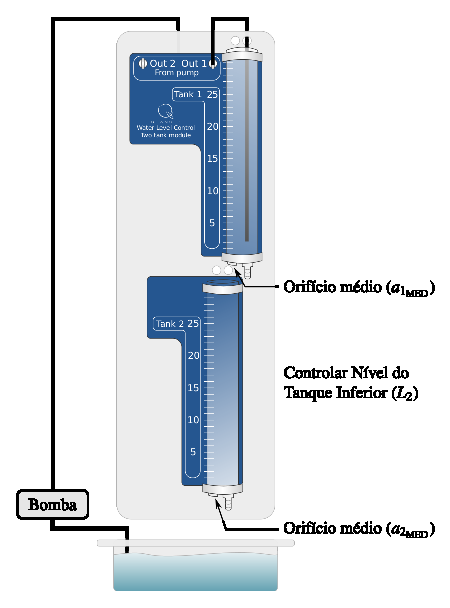
\includegraphics[width=0.31\textwidth]{imgs/sistema/eps/config_fab_2}
    \label{fig:config_fab_2}
}
\subfigure[Configuração 3]
{
    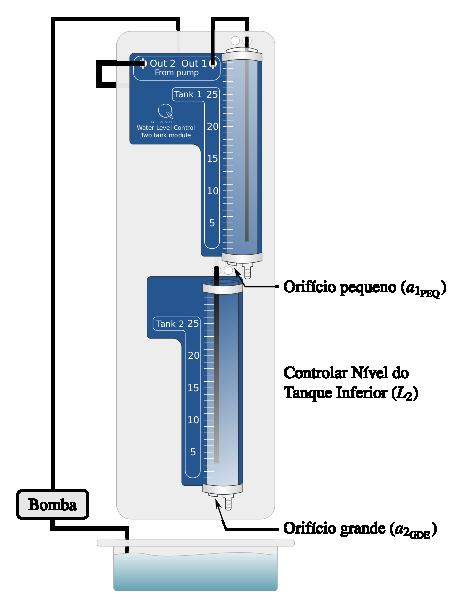
\includegraphics[width=0.31\textwidth]{imgs/sistema/eps/config_fab_3}
    \label{fig:config_fab_3}
}
\caption{Configurações sugeridas pelo fabricante.}
\label{fig:config_fab}
\end{figure}

Na primeira configuração deseja-se controlar o nível de $T_1$ ($L_1$) através de
uma alimentação direta, não fazendo uso do segundo tanque. Na segunda
configuração deseja-se controlar o nível de $T_2$ ($L_2$) a partir de uma
alimentação indireta em $T_1$. Assim, $T_2$ é alimentado a partir da água que
escoa de $T_1$ pelo orifício $a_1$. Por fim, na terceira configuração, deseja-se
controlar o nível de $T_2$ a partir da alimentação indireta de $T_1$ e da
alimentação direta de $T_2$. Para isso, faz-se uso dos dois orifícios de
entrada.

\Glossary{$L_1$}{Nível do tanque superior}
\Glossary{$L_2$}{Nível do tanque inferior}

Em todos os casos pode-se perceber que o sistema se comporta como um sistema de
uma única entrada, que é a tensão de alimentação da bomba, e uma única saída
({\it Single Input and Single Output} -- SISO), que pode ser $L_1$ ou $L_2$,
dependendo da configuração.

\Glossary{SISO}{{\it Single Input and Single Output}}

% TODO O controlador atua enviando um sinal de tensão para bomba... -3 a 3 =>
%Amplificador => -15 a 15

\subsection{Modelo matemático}

Como os dois tanques possuem mesma área de secção transversal ($A_1 = A_2$), a
dinâmica dos dois tanques será semelhante. Entretanto, encontrar um modelo
matemático que descreva adequadamente a dinâmica desses tanques não é algo tão
simples, visto que as equações gerais de movimento e energia que descrevem o
escoamento de fluidos são bastante complicadas \cite{dorf:2009}.

Assim sendo, é preciso que sejam feitas algumas hipóteses fundamentais.
Admite-se que a água no tanque é incompressível e que o escoamento é
não-viscoso, não-rotacional e regular. Cada uma dessas características serão
descritas a seguir baseadas na argumentação exposta em \citeasnoun{dorf:2009}.

Diz-se que um fluido é incompressível quando este possui uma massa específica
constante. Entretanto, sabe-se que todo fluido é compressível em certo grau e
que o fator de compressibilidade $k$ é uma medida de sua compressibilidade.
Quanto menor o valor de $k$, menor é a compressibilidade indicada para aquele
fluido. O ar, que é um fluido compressível, possui um fator de compressibilidade
$k_{\text{ar}} = 0,98\ \text{m}^2/\text{N}$, enquanto que a água tem um fator de
compressibilidade de $k_{\text{H}_2\text{O}} = 4,9 \times 10^{-10}\
\text{m}^2/\text{N} = 50 \times 10^{-6}\ \text{atm}^{-1}$. Em outras palavras,
um dado volume de água diminui em 50 milionésimos de seu volume original para um
aumento de uma atmosfera na pressão. Desse modo, a hipótese de que a água é
incompressível é valida para o sistema em questão.

Já a viscosidade de um fluido é dada pelo seu coeficiente de viscosidade $\mu\
(\text{N}\cdotp \text{s}/\text{m}^2)$. Quanto maior esse coeficiente, mais
viscoso é o fluido. Como exemplo, o coeficiente de viscosidade em condições
normais à 20\textdegree C para o ar é $\mu_{\text{ar}} = 0,178 \times 10^{-4}\
\text{N}\cdotp \text{s}/\text{m}^2$ enquanto que para a água
$\mu_{\text{H}_2\text{O}} = 1,054 \times 10^{-3}\ \text{N}\cdotp
\text{s}/\text{m}^2$. Assim, a água é cerca de 60 vezes mais viscosa que o ar.
Vale salientar que a viscosidade depende principalmente da temperatura e não da
pressão. Para efeitos de comparação, a água à 0\textdegree C é 2 vezes mais
viscosa que a água à 20\textdegree C. Com fluidos de baixa viscosidade como o ar
e a água, os efeitos do atrito são importantes apenas nas camadas de fronteira e
em uma fina camada adjacente à parede do reservatório e da tubulação de saída.
Assim, pode-se desprezar a viscosidade no desenvolvimento do modelo.

\Glossary{$\mu_{\text{ar}}$}{Coeficiente de viscosidade do ar}
\Glossary{$\mu_{\text{H}_2\text{O}}$}{Coeficiente de viscosidade da água}

Se cada elemento do fluido em cada ponto do escoamento não tem velocidade
angular com relação a esse ponto, o fluxo é denominado não-rotacional. Admita
que a água no tanque é não-rotacional. Logo, para um fluido não-viscoso, um
fluxo inicialmente não-rotacional permanece não-rotacional.

Por fim, o fluxo de água é dito regular se a velocidade em cada ponto é
constante com o tempo. Isso não implica necessariamente que a velocidade seja a
mesma em cada ponto, mas sim que em qualquer ponto a velocidade não mude com o
tempo. Condições de regime regular podem ser atingidas em velocidades baixas do
fluido. Admita então que há condições de fluxo regular. Observa-se entretanto
que se a área de abertura de saída fosse muito grande, o fluxo através do
reservatório não seria lento o suficiente para o estabelecimento das
condições de regime regular o que faria com que o modelo não conseguisse
predizer o fluxo do fluido de maneira exata.

Tendo esclarecido essas condições, para se obter o modelo matemático do fluido
dentro do reservatório emprega-se os princípios básicos da ciência e da
engenharia, como o princípio da conservação da massa. Assim, a massa de água em
qualquer instante de tempo é dada pela Eq. \ref{eq:conserv}.

\begin{equation}\label{eq:conserv}
m = \rhoagua\ AL
\end{equation}

\noindent em que $\rho_{\tiny \text{\tiny H}_2\text{\tiny O}}$ é a massa
específica da água, $A$ a área de secção transversal do reservatório e $L$ a
altura de água no reservatório. Tomando a derivada temporal de $m$ na Eq.
\ref{eq:conserv}, tem-se:

\begin{equation}
\dot{m} = \rhoagua\ A\dot{L}
\end{equation}

\noindent na qual utilizou-se o fato do fluido ser incompressível (ou seja,
$\dot{\rho} = 0$). Como a área de secção transversal não varia com o tempo, a
mudança de massa no reservatório é igual a massa que entra menos a massa que
deixa o tanque, logo:
 
\begin{equation}\label{eq:mudanca_massa}
\dot{m} = \rhoagua\ A\dot{L} = 
            Q_{\text{\tiny IN}} - 
\underbrace{\rhoagua\ a\upsilon_{\text{\tiny OUT}}}_
           {Q_{\text{\tiny OUT}}}
\end{equation}

\noindent em que $Q_{\text{\tiny IN}}$ é a vazão de entrada de massa em regime
permanente, $a$ é a área do orifício de saída e $\upsilon_{\text{\tiny OUT}}$ é
a velocidade de saída do fluido, que é uma função da altura da água. Da equação
de Bernoulli \cite{houghton:2002}, tem-se:

\begin{equation}
P_{\text{\tiny IN}} + 
\frac{1}{2}\rhoagua\ {\upsilon_{\text{\tiny IN}}}^2 +
\rhoagua\ gL
=
\frac{1}{2}\rhoagua\ {\upsilon_{\text{\tiny OUT}}}^2 +
P_{\text{\tiny OUT}}
\end{equation}

\noindent em que $\upsilon_{\text{\tiny IN}}$ é a velocidade da água na entrada
do reservatório e $P_{\text{\tiny IN}}$ e $P_{\text{\tiny OUT}}$ são as pressões
na entrada e na saída, respectivamente. Mas $P_{\text{\tiny IN}}$ e
$P_{\text{\tiny OUT}}$ são iguais à pressão atmosférica e a área de $a$ é
suficientemente pequena ($a \approx A/85$, considerando o orifício de saída
médio) para que a água escoe vagarosamente e a velocidade $\upsilon_{\text{\tiny
IN}}$ seja desprezível. Assim, a equação de Bernoulli fica reduzida a:

\begin{equation}\label{eq:bernoulli_red}
\upsilon_{\text{\tiny OUT}} = \sqrt{2gL}
\end{equation}

Além disso, segundo \citeasnoun{apkarian:1999}, a vazão de entrada
$Q_{\text{\tiny IN}}$ depende apenas da constante da bomba e da tensão à ela
aplicada, podendo ser positiva, quando a água é sugada do reservatório e
injetada no tanque, ou negativa quando a água é sugada do tanque e devolvida ao
reservatório. Assim:

\begin{equation}\label{eq:vazao_ent}
Q_{\text{\tiny IN}} = K_mV_p
\end{equation}

Substituindo então as Eqs. \ref{eq:bernoulli_red} e \ref{eq:vazao_ent} na Eq.
\ref{eq:mudanca_massa} e resolvendo para $\dot{L}$, tem-se:

\begin{equation}\label{eq:}
\dot{L} = -\left[\frac{a}{A}\sqrt{2g}\right]\sqrt{L} + 
          \frac{1}{\rhoagua\ A}K_mV_p
\end{equation}

% Continuar a partir do Dorf (eq 4.3 daqui do texto para obter Q_out)

\begin{comment}
 , exceto pelo fato de que a vazão de
entrada de $T_2$ irá depender apenas da vazão de entrada e da vazão de saída
de cada tanque. Entretanto, a vazão de saída da bomba

 Assim, as configurações
são estabelecidas de acordo com os orifícios de saída dos tanques e dos
orifícios de saída das bomba.

Mas, para isso, algumas considerações devem ser
feitas conforme demonstrado a seguir.

% TODO mostrar características expostas no dorf

Com o intuito de tornar a aplicação mais genérica, o sistema
original foi modificado introduzindo uma nova bomba, possibilitando novas
configurações, tais como aquelas representadas pela Fig.
\ref{fig:configuracoes}. 

Na primeira configuração (Fig. \ref{configuracoes_a}) as saídas duas bombas
estão dispostas de maneira individual com relação aos tanques. Já na segunda
configuração, as saídas estão posicionadas no tanque superior.

%Tal modificação faz com que o sistema se torne do tipo MIMO ({\it Multiple
%Input and Multiple Output})

Dessa forma, o sistema passa a ser composto por dois tanques e duas bombas, no
qual a água que sai do primeiro tanque é despejada no segundo tanque
\end{comment}

% ------------------------------------------------------------------------------
\section{Limitações do processo}

% ------------------------------------------------------------------------------
\section{Simulações de falhas}

% ------------------------------------------------------------------------------
\section{Estruturas neurais escolhidas}

% ------------------------------------------------------------------------------
\section{Esquemas de identificação}

% ------------------------------------------------------------------------------
\subsection{Proposta 1 -- Identificação global}

% ------------------------------------------------------------------------------
\subsection{Proposta 2 -- Identificação individual}

% ------------------------------------------------------------------------------
\section{Esquemas de detecção}

% ------------------------------------------------------------------------------
\subsection{Proposta 1 -- Comitê de especialistas}

% ------------------------------------------------------------------------------
\subsection{Proposta 2 -- Detecção global}

\mychapter{Resultados parciais}
\label{cap:resultados}

% Dados para as simulações da qualificação
% Tempo de simulação de 105 segundos (totalizando 00:01:45)
% Valores utilizados => Observar folha


% Montar tabela com os valores dos parametros alterados para o treinamento e
% para a validação das falhas. Exemplo:
% 
% FAVK => km_treinamento = (0.7 a 1.1)*km_original (PRBS)
%         km_validacao = (0.75 a 1.05)*km_original (PRBS) => nao precisa
%                                                            especificar o valor
%                                                            exato, mas dizer
%                                                            que estava dentro
%                                                            da faixa do
%                                                            treinamento
%         km_resultado = (0.75)*km_original (Fixo)
%
% FSeDG => ganho_treinamento = (1 +- 0.2)*ganho_original (PRBS)
%          ganho_validacao = (1 +- 0.15)*ganho_original (PRBS)
%          ganho_resultado = 0.8*ganho_original (fixo)
%


% Mostrar que foram feitos 3 conjuntos de validacao e depois foram escolhidas as
% melhores redes => Mostrar tabelas com Falso positivo e falso negativo


% Quando for falar sobre o número de regressores escolhidos => Dizer que
% considere que os regressores estão representados internamente ao "sistema de
% identificação" e ao "sistema de DDF" na figura da composição do sistema (final
% do cap:sistema)

\begin{comment}
Neste capítulo será realizada uma análise comparativa dos resultados obtidos nas
duas propostas do sistema de DDF. Ao final, do capítulo a melhor estrutura será
escolhida para que seja feita uma análise mais detalhada dos resultados.
\end{comment}

Neste capítulo serão analisados os resultados parciais obtidos a partir da
implementação da segunda proposta do sistema de DDF. Para isso, em um primeiro
momento será mostrado como se deu a coleta dos dados de treinamento e validação
das redes especialistas e em seguida será feita uma comparação de desempenho. Ao
final do capítulo as melhores estruturas serão selecionadas para que se realize
uma análise um pouco mais detalhada acerca da detecção das falhas.

% ------------------------------------------------------------------------------
\section{Coleta dos dados}
Tanto para o processo de identificação quanto para o processo de detecção, o
primeiro passo a ser dado é a obtenção das amostras experimentais para o
treinamento supervisionado das redes neurais de inferência e de detecção.

Dessa maneira, realizou-se a coleta dos dados a partir da estimulação do sistema
simulado através da aplicação de sinais binários pseudo aleatórios ({Pseudo
Random Binary Signals} -- PRBS) à referência de cada um dos tanques e aos
parâmetros do sistema que simulam as falhas. Para a identificação, a faixa de
valores aplicados se deu do nível mínimo (zero) ao máximo (trinta). Já para a
detecção das falhas, os valores foram aplicados conforme Tab.
\ref{tab:valores_treinamento}. Nessa tabela os valores mínimos e máximos são
multiplicados pelo valor padrão e aplicados ao modelo. A última coluna mostra
qual será a representatividade da mudança dos valores.

\begin{table}[htb]
\caption{Valores aplicados para o treinamento das redes neurais de detecção.}
\label{tab:valores_treinamento}
\vspace{0.25cm}
\centering
\begin{threeparttable}
\begin{tabular}{|c|c|c|c|c|}
\hline
{\bf Falha} & {\bf Valor padrão} & {\bf Mínimo} & {\bf Máximo} & 
{\bf Representatividade}\\
\hline
\hline
FSeDG & 0,16\tnote{$*$} & 
0,8 & 1,2 & Até $\pm 6$ cm\\
\hline
FSeDO & 1,0 & -3,0 & 3,0 & Até $\pm 3$ cm\\
\hline
FSeSR & 1,0 & -0,03 & 0,03 & Até $\pm 9$ cm\\
\hline
FSeQ & 1,0 & 0,0 & 0,0 & -- \\
\hline
\hline
FADG & 1,0 & 0,8 & 1,0 & Até -3 Volts\\
\hline
FADO & 1,0 & -1,0 & 0,0 & Até -1 Volts\\
\hline
FASR & 1,0 & -0,03 & 0,03 & Até $\pm 0,45$ Volts\\
\hline
FAVK & $K_m$ & 0,7 & 1,1 & --\\
\hline
FAQ & 1,0 & 0,0 & 0,0 & --\\
\hline
\hline
FSiVzT & $a_{i_{\text{\tiny MED}}}$ & 
0,25 & 0,75 & 25 a 75\% de $a_{i_{\text{\tiny MED}}}$\\
\hline
FSiVrOS & $a_{i_{\text{\tiny MED}}}$ & 
0,75 & 1,25 & $\pm 25\%$ de $a_{i_{\text{\tiny MED}}}$\\
\hline
FSiVrGMP & 5,0\tnote{$*$} & 
0,8 & 1,0 & Até -3 Volts\\
\hline
FSiEOS & $a_{i_{\text{\tiny MED}}}$ & 
0,0 & 0,5 & --\\
\hline
\end{tabular}
\begin{tablenotes}
\item [$*$] Estabelecido pelo manual do fabricante.
\end{tablenotes}
\end{threeparttable}
\end{table}

Perceba que nas falhas dos atuadores, as tensões a serem aplicadas podem vir a
danificar a bomba. Por esse motivo não seria viável obter as amostras do
processo real, mas sim a partir de uma simulação.

Os sinais pseudo aleatórios gerados se mantiveram dentro dos limites
estabelecidos durante todo o intervalo de tempo da simulação. Para o processo de
identificação foram obtidas 6000 (seis mil) amostras, equivalentes à 10 (dez)
minutos de simulação. Já para a detecção o processo foi simulado durante 20
(vinte) minutos, o que correspondeu a obtenção de 12000 (doze mil) amostras.

De posse dos valores obtidos, iniciou-se a fase de treinamento das RNAs. Todas
as redes foram treinadas de modo {\it offline} com o {\it toolbox} de redes
neurais do {\it software} matemático Matlab\reg\ utilizando o algoritmo LMA. Ao
final de cada etapa de treinamento as redes eram submetidas à testes de
validação para que se fosse possível avaliar a capacidade de generalização.

% ------------------------------------------------------------------------------
\section{Análise das RNAs}
Para que se fossem estabelecidos critérios avaliativos significantes, ou seja,
para que existisse um número representativo, diversas redes neurais foram
treinadas com diferentes configurações considerando o número de neurônios na
camada oculta e a ordem do modelo. O número de redes treinadas corresponde
aquele especificado no final da Tab. \ref{tab:treinamentos}. 

\begin{table}[htb]
\centering
\caption[Número de redes neurais treinadas]{Número de redes neurais treinadas de
acordo com a ordem do modelo e o número de neurônios na camada oculta.}
\label{tab:treinamentos}
\vspace{0.25cm}
\begin{tabular}{|c|c|c|c|c|}
\hline
% Linha 1
\multirow{2}{*}{\bf Proposta} & 
\multirow{2}{*}{\bf Ordem} & 
{\bf Neurônios na} & 
{\bf Número de} & 
\multirow{2}{*}{\bf Total}\\
% Linha 2
& & {\bf camada oculta} & {\bf redes treinadas} &\\
\hline
\hline
\multicolumn{5}{|l|}{{\bf Identificação}}\\
\hline
\hline
\multirow{3}{*}{1} & 2 & 6/8/10 & \multirow{3}{*}{6} & \multirow{3}{*}{54}\\
\cline{2-3}
& 3 & 8/12/16 & &\\
\cline{2-3}
& 4 & 10/16/22 & &\\
\hline
\multirow{3}{*}{2} & 2 & 2/4/6 -- 6/8/10 & 
\multirow{3}{*}{6} & \multirow{3}{*}{108}\\
\cline{2-3}
& 3 & 4/6/8 -- 8/12/16 & & \\
\cline{2-3}
& 4 & 6/8/10 -- 10/16/22 & & \\
\hline
\multicolumn{5}{|l|}{{\bf Detecção}}\\
\hline
\hline
\multirow{3}{*}{2} & 2 & 8/12/16 & 
\multirow{3}{*}{6/falha} &
\multirow{3}{*}{702}\\
\cline{2-3}
& 3 & 14/18/22 & &\\
\cline{2-3}
& 4 & 20/24/28 & &\\
\hline
\hline
\multicolumn{4}{|r|}{{\bf Total}} & 864\\
\hline
\end{tabular}
\end{table}

Pode-se compreender essa tabela facilmente a partir de um exemplo: na primeira
proposta de identificação, considerando a linha de ordem igual 2, foram
treinadas 6 redes neurais cada vez que o número de neurônios na camada oculta
era alterado (6, 8 ou 10 neurônios). Assim, para cada ordem eram treinadas 18
redes neurais. Como foram testadas três ordens distintas, tem-se um total de 54
redes para a primeira proposta.

As únicas observações a serem feitas são que, na segunda proposta de
identificação existiam duas redes neurais a serem treinadas em cada etapa de
treinamento, conforme Fig. \ref{fig:ident_proposta_2}, e que a segunda proposta
de detecção considera-se um conjunto de 13 (treze) redes especialistas, sendo
uma para cada falha, conforme Fig. \ref{fig:detec_prop_2}. Em virtude desses
aspectos, o número de redes treinadas dobra da primeira para a segunda proposta
de identificação e é multiplicado por um fator de treze para a segunda proposta
de detecção.

% ------------------------------------------------------------------------------
\subsection{Identificação}

% ------------------------------------------------------------------------------
\subsection{Detecção de falhas}

% ------------------------------------------------------------------------------
\section{Melhores redes}

% ------------------------------------------------------------------------------
\section{Composição final}

% ------------------------------------------------------------------------------
\section{Detecções}

% ------------------------------------------------------------------------------
\section{Comparação das propostas}

% Falhas nos sensores ..........................................................
\begin{figure}[htb]
\footnotesize
\centering
\input{scripts/fsedg}
\vspace{1cm}
\caption{FSeDG (80\%)}
\label{fig:fsedg}
\end{figure}

\begin{figure}[htb]
\footnotesize
\centering
\input{scripts/fsedo}
\vspace{1cm}
\caption{FSeDO (-2 cm)}
\label{fig:fsedo}
\end{figure}

\begin{figure}[htb]
\footnotesize
\centering
\input{scripts/fsesr}
\vspace{1cm}
\caption{FSeSR ($\pm 2\%$)}
\label{fig:fsesr}
\end{figure}

\begin{figure}[htb]
\footnotesize
\centering
\input{scripts/fseq}
\vspace{1cm}
\caption{FSeQ (Ganho = 0)}
\label{fig:fseq}
\end{figure}

% Falhas nos atuadores .........................................................
\begin{figure}[htb]
\footnotesize
\centering
\input{scripts/fadg}
\vspace{1cm}
\caption{FADG (80\%)}
\label{fig:fadg}
\end{figure}

\begin{figure}[htb]
\footnotesize
\centering
\input{scripts/fado}
\vspace{1cm}
\caption{FADO (-0,5 Volts)}
\label{fig:fado}
\end{figure}

\begin{figure}[htb]
\footnotesize
\centering
\input{scripts/fasr}
\vspace{1cm}
\caption{FASR ($\pm 2\%$)}
\label{fig:fasr}
\end{figure}

\begin{figure}[htb]
\footnotesize
\centering
\input{scripts/favk}
\vspace{1cm}
\caption{FAVK (75\%)}
\label{fig:favk}
\end{figure}

\begin{figure}[htb]
\footnotesize
\centering
\input{scripts/faq}
\vspace{1cm}
\caption{FAQ (Ganho = 0)}
\label{fig:faq}
\end{figure}

% Falhas no sistema ............................................................
\begin{figure}[htb]
\footnotesize
\centering
\input{scripts/fsivzt}
\vspace{1cm}
\caption{FSiVzT ($a_{\tiny VZ} = \frac{a_{\tiny MED}}{2}$)}
\label{fig:fsivzt}
\end{figure}

\begin{figure}[htb]
\footnotesize
\centering
\input{scripts/fsivros}
\vspace{1cm}
\caption{FSiVrOS ($a' = \frac{a_{\tiny MED}}{2}$)}
\label{fig:fsivros}
\end{figure}

\begin{figure}[htb]
\footnotesize
\centering
\input{scripts/fsivrgmp}
\vspace{1cm}
\caption{FSiVrGMP (90\%)}
\label{fig:fsivrgmp}
\end{figure}

\begin{figure}[htb]
\footnotesize
\centering
\input{scripts/fsieos}
\vspace{1cm}
\caption{FSiEOS (25\%)}
\label{fig:fsieos}
\end{figure}

\mychapter{Conclusões}
\label{cap:conclusoes}

% ------------------------------------------------------------------------------
\section{\ldots}


\backmatter
% Apêndices --------------------------------------------------------------------
%\appendix
%\input{apendices/codigos}

% Bibliografia -----------------------------------------------------------------
\addcontentsline{toc}{chapter}{Referências Bibliográficas}
\bibliographystyle{ppgeec}
\bibliography{bibliografia}

% Fim do documento .............................................................
\end{document}
